\newpage
\section{Aufgabe 3}
\label{sec:a1}
\subsection{a)}
\label{subsec:a1}

Die Messwerte aus der Datei $aufg\_a.csv$ sollen mit Hilfe der
Methode der kleinsten Quadrate an ein Polynom 6. Grades
\begin{align}
p(x)=a_1+a_2x+a_3x^2+ a_4x^3+a_5x^4+a_6x^5+a_7x^6
\end{align}
gefittet werden.
Dafür wird die Designmatrix A für die Messewerte bestimmt
 und über die Formel
 \begin{align}
\vec a =(A^TA)^{-1}A\vec y
 \end{align}
folgen die Koeffizienten die in der Tabelle \ref{tab:a} aufgelistet sind.
In der Abbildung \ref{fig:a} sind die Messwerte und das Polynom
dargestellt.
\begin{table}
  \caption{Koeffizienten des Polynoms 6.Grades für den Fit.}
  \label{tab:a}
  \begin{tabular}{c c c c c c c}
\toprule
    $a_1 $&$ a_2 $&$ a_3 $&$  a_4 $&$  a_5 $&$ a_6 $&$a_7$\\
\midrule
$-6,7\cdot10^{-2} $&$ 6,1\cdot10^{-1} $&$ -5,1\cdot10^{-1} $&$ 2,1\cdot10^{-1} $&$   -4,5\cdot10^{-2} $&$ 4,8\cdot10^{-3} $&$  -1,9\cdot10^{-4}$ \\
\bottomrule
  \end{tabular}
\end{table}


\begin{figure}
  \centering
  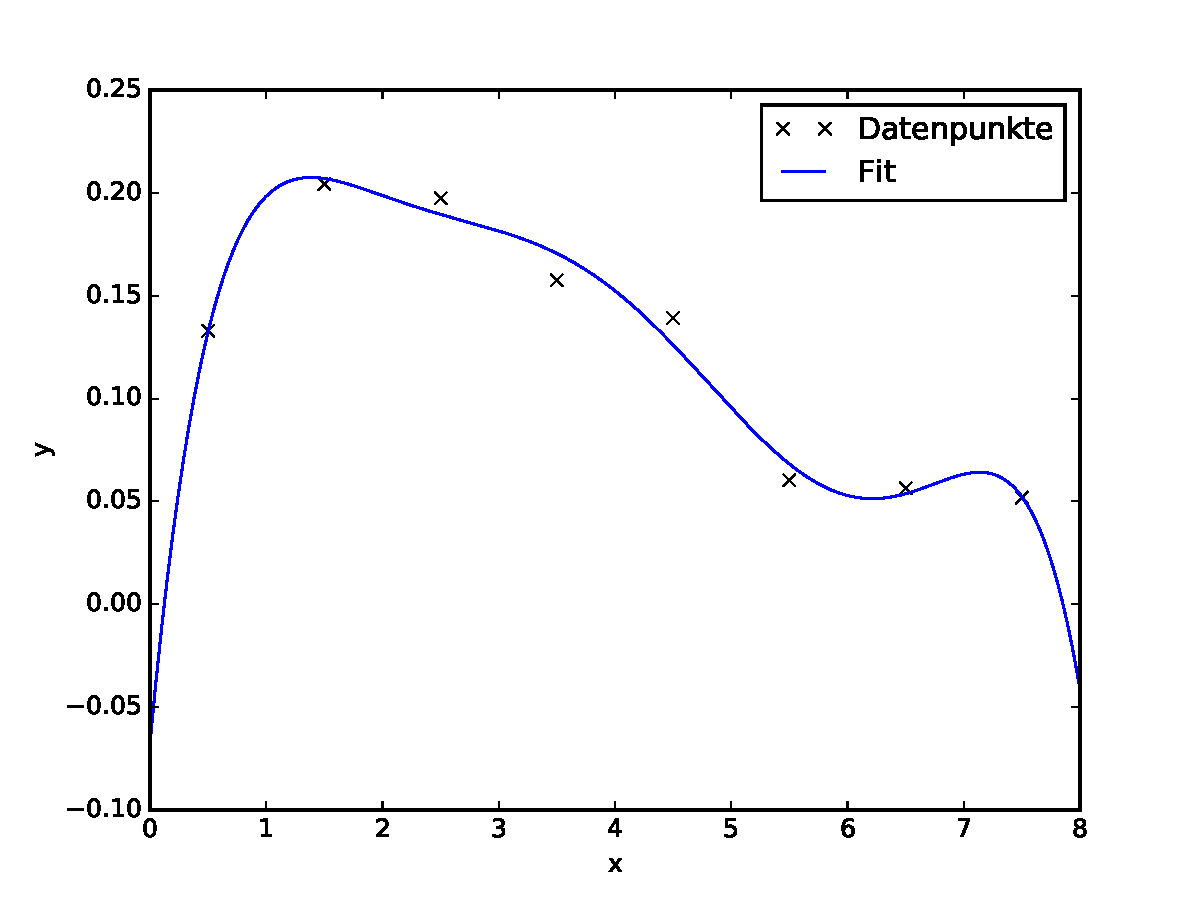
\includegraphics[width=0.7\textwidth]{Fit.pdf}
  \caption{Messwerte und Fit für die Messwerte.}
  \label{fig:a}
\end{figure}


\FloatBarrier
\subsection{b)}
\label{subsec:a1b}
Nun soll über eine Reguariserung $(\Gamma=\sqrt{\lambda}CA)$ in den Fit mit
eingehen.
Die unterschiedlichen Regularisierungsstärken sind
 $\lambda \in (0.1,0.3,0.7,3,10)$.
Die Koeffizienten die sich für die unterschiedlichen
Regularisierungsstärken sind in der Tabelle\ref{tab:b} und
die dazugehörigen Graphen in der Abbildung \ref{fig:b} zu finden.
\begin{table}
  \caption{Koeffizienten des Polynoms 6.Grades für den Fit bei underschiedlichen Regularisierungsstärken $\lambda$.}
  \label{tab:b}
  \begin{tabular}{ c c c c c c c c}
\toprule
  $\lambda$  & $a_1 $&$ a_2 $&$ a_3 $&$  a_4 $&$  a_5 $&$ a_6 $&$a_7$\\
\midrule
$0,1  $  & $5,3\cdot10^{-02}$&$ 2,6\cdot10^{-01} $&$ -1,9\cdot10^{-01} $&$ 7,7\cdot10^{-02} $&$-1,7\cdot10^{-02} $&$1,9\cdot10^{-03} $&$-8,1\cdot10^{-05}$\\
$0,3  $  & $1,1\cdot10^{-01}$&$ 1,1\cdot10^{-01} $&$ -6,4\cdot10^{-02} $&$ 2,5\cdot10^{-02} $&$-6,3\cdot10^{-03} $&$7,9\cdot10^{-04} $&$-3,6\cdot10^{-05}$\\
$0,7  $  & $1,4\cdot10^{-01}$&$ 4,4\cdot10^{-02} $&$ -1,7\cdot10^{-02} $&$ 6,5\cdot10^{-03} $&$-2,4\cdot10^{-03} $&$3,6\cdot10^{-04} $&$-1,8\cdot10^{-05}$\\
$3    $  & $1,7\cdot10^{-01}$&$ 8,0\cdot10^{-03} $&$ -1,1\cdot10^{-03} $&$-1,1\cdot10^{-04} $&$-4,9\cdot10^{-04} $&$1,1\cdot10^{-04} $&$-6,0\cdot10^{-06}$\\
$10   $  & $1,7\cdot10^{-01}$&$ 2,1\cdot10^{-03} $&$ -2,1\cdot10^{-03} $&$-1,9\cdot10^{-04} $&$-1,4\cdot10^{-04} $&$3,9\cdot10^{-05} $&$-2,3\cdot10^{-06}$\\
\bottomrule
  \end{tabular}
\end{table}


\begin{figure}
  \centering
  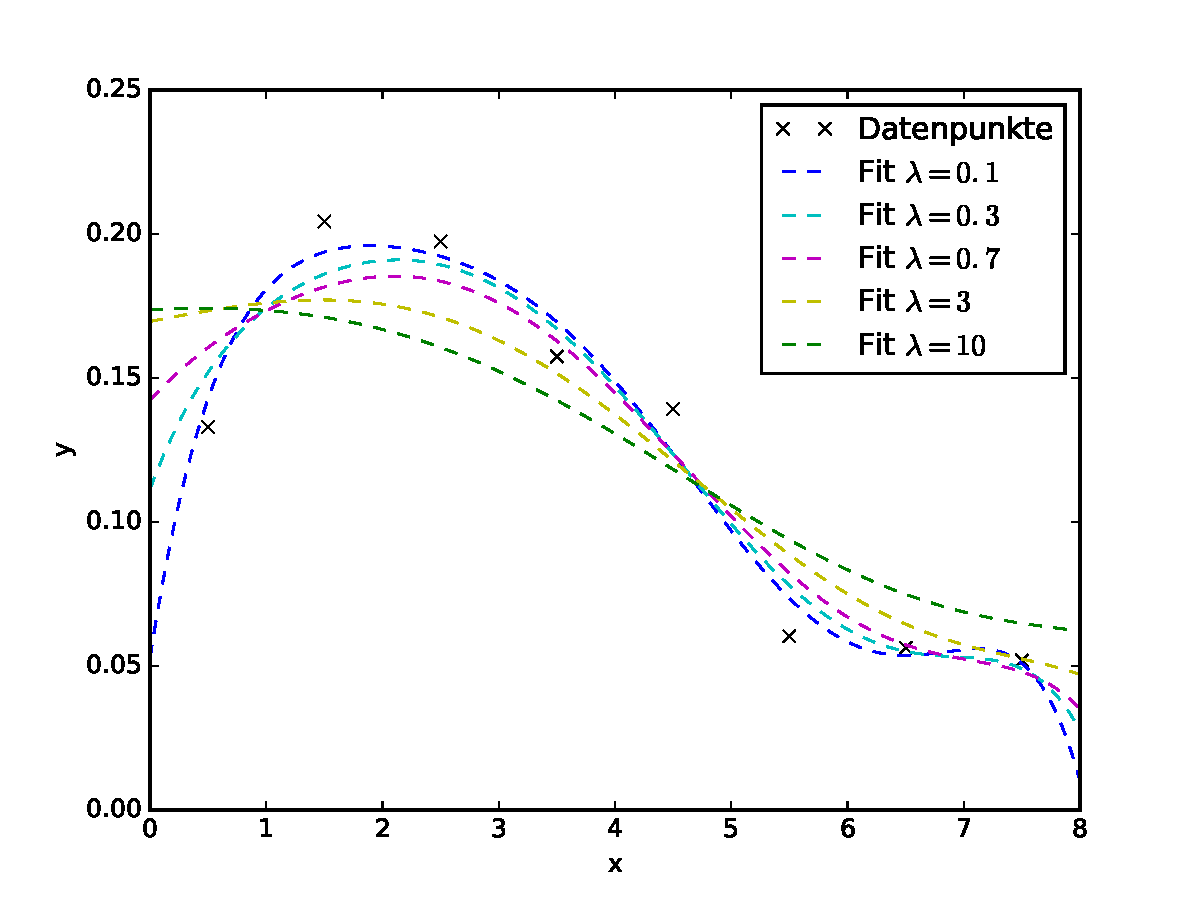
\includegraphics[width=0.7\textwidth]{Fit_b).pdf}
  \caption{Messwerte und
   Fit bei underschiedlichen Regularisierungsstärken $\lambda$.}
  \label{fig:b}
\end{figure}



\FloatBarrier
\subsection{c)}
\label{subsec:a1c}
Diesmal werden die Daten aus der Datei $aufg\_c.csv$ verwendet.
Die Messungen für einen x-wert werden gemittelt und
der Mittelwertfehler wird mit der Formel
\begin{align}
  \sigma=\sqrt{\frac{1}{n-1}\sum_{i=1}^n(x_i-\overline{x})^2}
\end{align}
berechnet.
Die Mittelwerte und die entsprechenden Fehler sind in
der Tabelle \ref{tab:mitt} zu finden.

\begin{table}
  \centering
  \caption{Mittelwerte von $y$ und Mittelwertfehler für ensprechende $x$ Werte.}
  \label{tab:mitt}
  \begin{tabular}{ c c c}
\toprule
 $x$ & $\overline{y}$ & $\sigma_y $\\
  \midrule
  $0,50$ & $0,12 $ & $ 0,02$\\
  $1,50$ & $0,18 $ & $0,03 $\\
  $2,50$ & $0,20 $ & $0,03 $\\
  $3,50$ & $0,16 $ & $0,03 $\\
  $4,50$ & $0,12 $ & $0,02 $\\
  $5,50$ & $0,09 $ & $0,02 $\\
  $6,50$ & $0,07 $ & $0,01 $\\
  $7,50$ & $0,06 $ & $0,01 $\\
\bottomrule
  \end{tabular}
\end{table}

Über die Mittelwertfehler kann eine Gewichtsmatrix $W$
definiert werden mit dieser und der Formel
\begin{align}
  \vec a=(A^TWA)^{-1} A^T W \vec y
\end{align}
  können die Parameter für den Fit bestimmt werden.
  Diese sind in der Tabelle \ref{tab:c}
  aufgelistet und in der Abbildung \ref{fig:c}
  sind die berechneten Mittelwerte mit Fehler sowie der
  Fit enthalten.

  \begin{table}
    \caption{Koeffizienten des Polynoms 6.Grades für den Fit.}
    \label{tab:c}
    \begin{tabular}{c c c c c c c}
  \toprule
      $a_1 $&$ a_2 $&$ a_3 $&$  a_4 $&$  a_5 $&$ a_6 $&$a_7$\\
  \midrule
  $1,0\cdot 10^{-1} $&$   1,9\cdot 10^{-2} $&$   6,2\cdot 10^{-2} $&$  -3,8\cdot 10^{-2} $&$
  7,9\cdot 10^{-3} $&$ -7,3\cdot 10^{-04}  $&$ 2,6\cdot 10^{-5}$\\
  \bottomrule
    \end{tabular}
  \end{table}


  \begin{figure}
    \centering
    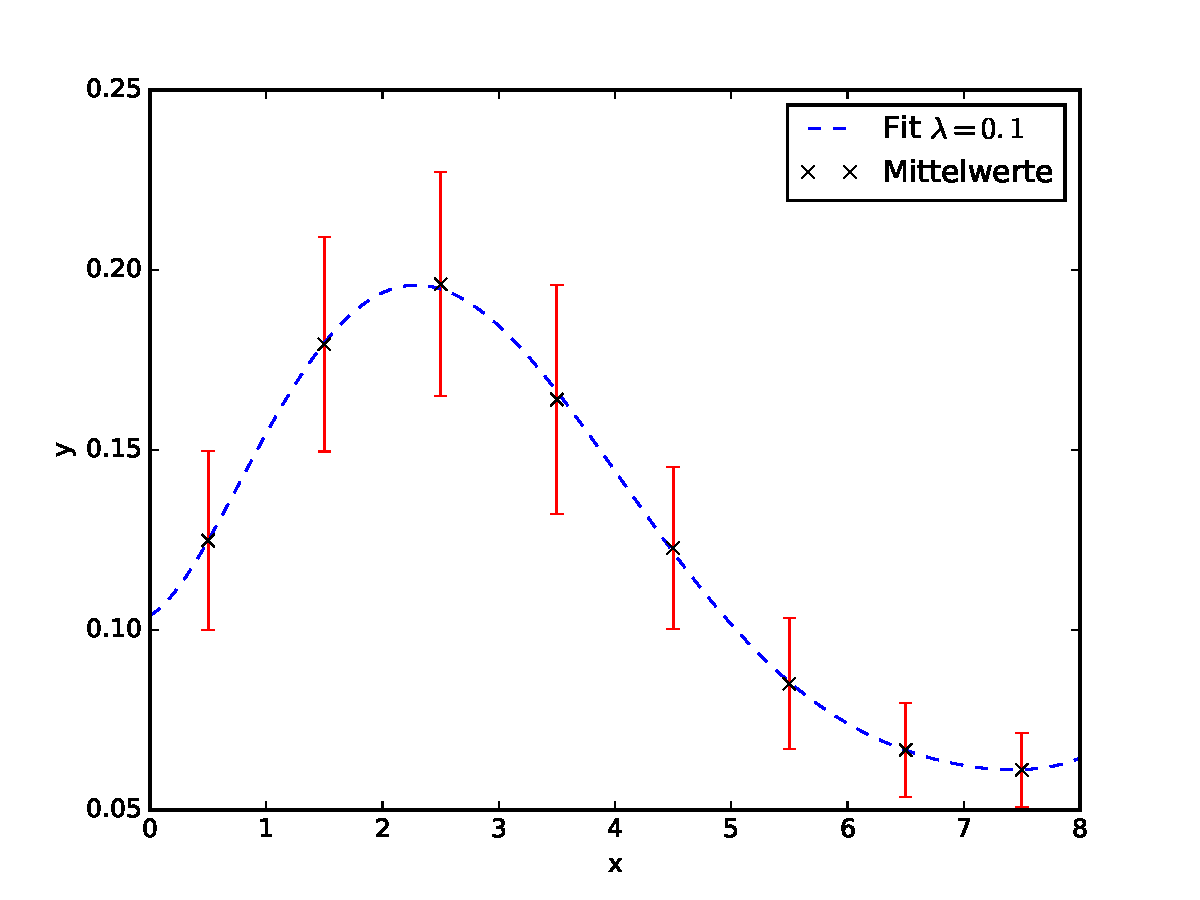
\includegraphics[width=0.7\textwidth]{Fit_c).pdf}
    \caption{Mittelwerte der Messwerte und deren Mittelwertfehler
     und Fit mit Hilfe einer Gewichtsmatrix.}
    \label{fig:c}
  \end{figure}
